% $Id: ScriptRW.tex,v 1.1 2008/01/31 18:04:17 dconway Exp $
\chapter{\label{chapter:ScriptRW}Script Reading and Writing}
\chapauthor{Darrel J. Conway}{Thinking Systems, Inc.}

GMAT stores mission modeling data in a text file referred to as a GMAT script file.  The scripting
language used in GMAT is documented in \cite{userGuide}.  This chapter describes the architecture of
the ScriptInterpreter subsystem, which is used to read and write these files.

GMAT scripts, like MATLAB scripts, are case sensitive.  In the sections that follow, script
elements, when they appear, will be written with the proper case.  That said, this chapter is not
meant to be a comprehensive text on GMAT scripting.  Script lines and portions of lines are
presented here for the purpose of describing the workings of the ScriptInterpreter and related
classes.

\section{\label{section:ReadingScript}Loading a Script into GMAT}

\begin{figure}[htb]
\begin{center}
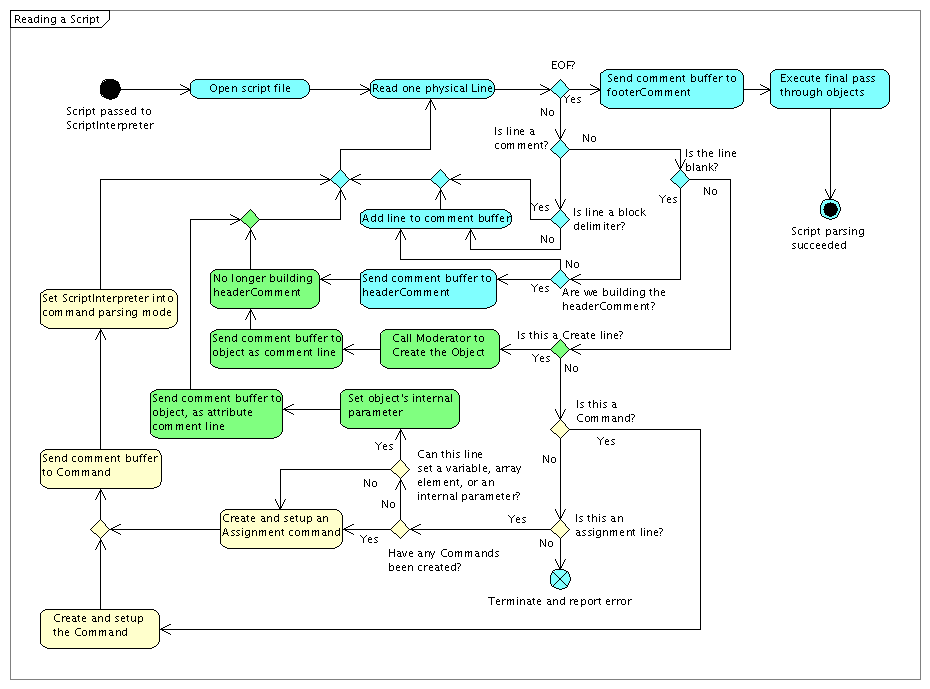
\includegraphics[430,319]{Images/ReadingaScript.png}
\caption{\label{figure:ReadingScriptFlow}Sequence Followed when Loading a Script into GMAT}
\end{center}
\end{figure}

Figure~\ref{figure:ReadingScriptFlow} shows the sequence followed when GMAT opens a script file and
reads it, constructing internal objects that model the behavior dictated by the script.  Some of the
detailed work performed in this process is dictated by the properties of the objects; the figure
provides the general flow through the process.  The figure is color coded to reflect three basic
groupings of actions taken while reading a script file.  The large scale flow through the
ScriptInterpreter system is colored blue; actions that affect configured objects are colored green,
and actions related to the time ordered Mission Sequence are colored yellow.  This figure shows a
fair amount of complexity; the section describing the subsystem classes breaks this complexity into
more manageable pieces.

When a user instructs GMAT to read a script, either from the command line or from the graphical
user interface, the Moderator receives an InterpretScript() command containing the name of the file
that needs to be read.  This command calls the Interpret() command on the ScriptInterpreter, which
uses the classes and methods provided in the Interpreter subsystem and described in this chapter,
to read the script and configure the objects described in it.

There are four types of physical lines in a script file: (1) comment lines, which start with a
percent sign (\%), (2) object definition lines, which start with the word ``Create'', (3) command
lines, which start with the text assigned to a GmatCommand class, and (4) assignment lines, which
optionally start with the word ``GMAT''\footnote{The GMAT keyword is automatically inserted on
assignment lines when a script is written.  The ScriptReadWriter class has an internal flag that
toggles this feature on and off when writing, so that future versions of GMAT can provide the
ability to turn this feature on or off.}. Comments can be appended on the end of script lines; when
that happens, all of the text following the percent sign comment delimiter is associated with the
line and referred to as an inline comment in this document.

The script file is read one ``logical block'' at a time, using the ScriptReadWriter helper class.  A
logical block consists of one or more physical lines in the script file.  Each logical block can
have three elements: one or more lines of opening comments (identified with leading \% characters),
an instruction that tells GMAT to do something, and an inline comment appended to the end of the
instruction.  Each logical block has at least one of these elements, but need not have all three.
Inline comments cannot exist on their own -- they require the instruction component.

The instruction element can be split up over multiple physical lines in the script file, as long as
each physical line is terminated by ellipsis~(...).  Inline comments for a multiline instruction
must be placed at the end of the last physical line of the block.  White space at the beginning
of each line of an instruction is discarded.  Lines that are continued using ellipsis markers pick
up an extra space in place of the ellipsis characters.  Instructions in a logical blocks can be
terminated with a semicolon; this character has no effect in GMAT\footnote{Semicolons are used in
MATLAB to suppress display of the result of the line of text.  Since GMAT scripts can be read in the
MATLAB environment, the GMAT scripting language allows, but does not require, a semicolon at the end
of an instruction.}.  Once a logical block has been read from the file using these rules, it is
analyzed to determine the type of information contained in the block.

The ScriptInterpreter treats comment lines that start with the sequence ``\texttt{
\%\nobreakdash-\nobreakdash-\nobreakdash-\nobreakdash-\nobreakdash-\nobreakdash-\nobreakdash-}''  as
a special type of comment, called a block delimiter. These lines are ignored by the
ScriptInterpreter when reading a script.  Details concerning comment handling are presented later
in this chapter, as are the detailed control flow procedures GMAT follows when working with scripts.

\subsection{\label{section:ScriptComments}Comment Lines}

Comments in GMAT scripts are started with the percent sign~(\%).  Comments can exist in one of two
different forms: either on individual lines, or inline with other GMAT scripting, as shown here:

\begin{quote}
\linenumbers[1]
\begin{verbatim}
%---------------------------------------------------------------------
%-----------             Spacecraft Components            ------------
%---------------------------------------------------------------------

% This is the main spacecraft in the mission.
Create Spacecraft mainSat     % Not to be confused with MaineSat
GMAT mainSat.X  = 42165.0     % Start at GEO distance
GMAT mainSat.Y  = 0.0
GMAT mainSat.Z  = 0.0
     % This is the velocity part.  I've intentionally made the
     % indentation ugly to make a point: leading white space is
     % preserved in comment lines.
GMAT mainSat.VX = 0.0         % But slower than a circular orbit
GMAT mainSat.VY = 1.40
GMAT mainSat.VZ = 0.95
\end{verbatim}
\nolinenumbers
\end{quote}

\noindent Lines~1-3 and lines~5 and~10-12 are individual comment lines.  Lines~6, 7 and~13 contain
inline comments.  The individual comment lines fall into two categories: lines~1-3 here are block
delimiter lines, denoted by the delimiter identifier at the start of each line, while lines~5
and~10-12 are user supplied comments.  The ScriptInterpreter inserts the block comments
automatically when a script is written, and skips over those comment lines when reading the script.
The user provided comments like lines~5 and~10-12 are stored with the data provided immediately
after those lines.  In this script snippet, for example, the comment ``\texttt{\% This is the main
spacecraft in the mission}'' is associated with the object creation line, and stored as an object
level comment for the Spacecraft named mainSat.  The comments on lines~10-12:

\begin{quote}
\linenumbers[10]
\begin{verbatim}
     % This is the velocity part.  I've intentionally made the
     % indentation ugly to make a point: leading white space is
     % preserved in comment lines.
\end{verbatim}
\end{quote}

\noindent are associated with the assignment line ``\texttt{GMAT mainSat.VX = 0.0}'', and
stored, including linebreaks, in the data member associated with the object parameter mainSat.VX.
Each entire line is stored, including the leading whitespace, so that the ScriptInterpreter can
reproduce the comment verbatim.

Inline comments are stored with the GMAT structure that most closely matches the comment line.
Hence the inline comment on line~6 is stored in the data member associated with the Spacecraft
mainSat, while the inline comments on lines~7 and~13 are stored incorresponding members of a
StringArray in that object that maps the comment to the corresponding spacecraft parameters:
mainSat.X and mainSat.VX for this example.

\begin{figure}[htb]
\begin{center}
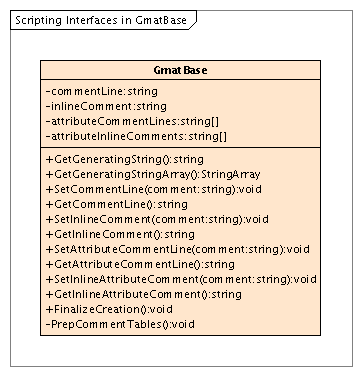
\includegraphics[220,229]{Images/ScriptingInterfacesinGmatBase.png}
% CommentInterfacesinGmatBase.png: 334x360 pixel, 72dpi, 12.77x11.08 cm, bb=0 0 334 360
\caption{\label{figure:GmatBaseCommentInterface}Scripting Interfaces in the User Classes}
\end{center}
\end{figure}

The ScriptInterpreter makes these associations when it finds comments in a script.  Comment lines
are buffered in the ScriptInterpreter, and written to the next resource encountered in the script
file.  The GmatBase class contains the data structures and interfaces needed to implement this
functionality.  These interfaces are shown in Figure~\ref{figure:GmatBaseCommentInterface}.

There are two additional types of comment blocks that GMAT manages.  Comments that occur at the
beginning and at the end of a script are saved in the ScriptInterpreter in case they are needed for
display on the GUI or when writing a script.  The header comment consists of all comment lines found
at the start of a script to the first blank line in the script. If an instruction is detected before
a blank line, the header comment is set to the empty string.  Similarly, the script's footer comment
consists of all comments that are found after the final instruction in the script.  If no comments
are found after the final instruction, the footer comment is set to the empty string.

\subsection{\label{section:ParsingObjectDefinitions}Object Definition Lines}

When the ScriptInterpreter detects an object definition instruction (starting with the word
``Create''), it breaks the line into three pieces: the initial ``Create'' keyword, the type name for
the object that needs to be created, and one or more names used for the created objects.  When
multiple objects are created on a single line, the object names are separated using
commas\footnote{Note that commas are required. This restriction comes from the interoperability
requirement between GMAT and MATLAB.  If the commas are omitted, then when MATLAB parses the line,
it creates a cell array for the elements following the Create keyword.  A similar constraint applies
to all script instructions when the blocks in the instruction exist outside of parentheses,
brackets, or braces.}.  Three examples of object definition are provided here:

\begin{quote}
\linenumbers[1]
\begin{verbatim}
Create Spacecraft MMSRef;
Create Spacecraft MMS1, MMS2, MMS3, MMS4;
Create Array squareArray[3, 3] notSquare[4, 7] vector[6]
\end{verbatim}
\end{quote}

\noindent The first script line here (``\texttt{Create Spacecraft MMSRef;}'') demonstrates basic
object creation. When the ScriptInterpreter parses this line, it calls the Moderator and instructs
it to create an instance of the Spacecraft class named MMSRef.  The Moderator calls the appropriate
factory (the spacecraft factory in this case) and obtains the object.  It then adds this object to
the configured objects, and returns the object pointer to the ScriptInterpreter. The
ScriptInterpreter validates the returned pointer, ensuring that the pointer is not NULL, performs
finalization on the object by calling the ``\texttt{FinalizeCreation()}'' method, and then moves to
the next line.  If no factory is available to create the object, the Moderator throws an exception
which the ScriptInterpreter handles.  The ScriptInterpreter throws an expection that is displayed to
the user, indicating the line number of the offending line, the nature of the error encountered,
and, in quotation marks, the text of the line that caused the error.

The second script line (``\texttt{Create Spacecraft MMS1, MMS2, MMS3, MMS4;}'') works
identically, calling the Moderator four consecutive times to create the four spacecraft named MMS1,
MMS2, MMS3, and MMS4.  Each object is created, validated by testing the returned pointer to
see if it is NULL, and finalized using \texttt{FinalizeCreation()}.  The ScriptInterpreter loops
through the list of requested objects, and performs this procedure one name at a time.

The array creation line (``\texttt{Create Array squareArray[3, 3] notSquare[4, 7] vector[6]}'')
requires a bit of additional parsing.  Arrays require the count of the number of rows and
columns\footnote{GMAT does not support matrices with more than 2 dimensions at this time.} in
the array before it can be constructed.  These counts are contained in square braces in the array
creation line.  Each array on the line has a separate field indicating this size.  If a user
specifies a single dimension for the array, as in the case of the array named \texttt{vector} in
this example, that dimension is the column count for the object: \texttt{vector} as specified here
is a 1 by 6 array.  Once the size parameters have been parsed, the ScriptInterpreter proceeds as
before: the Moderator is called and instructed to create an array with the desired dimensions.  This
array is created in the factory subsystem, added to the object configuration, and returned to the
ScriptInterpreter for pointer validation.  Once the pointer has been validated, the
ScriptInterpreter executed the \texttt{FinalizeCreation()} method on the new object, and then
proceeds to the next line of script.

\subsection{\label{section:ParsingCommands}Command Lines}

If the logical block is not an object definition line, the ScriptInterpreter next checks to see if
the line is a GMAT command.  GMAT commands all start with the keyword assigned to the specific
command; examples include \texttt{Propagate}, \texttt{For}, \texttt{Maneuver}, \texttt{Target}, and
\texttt{BeginFiniteBurn}.  A typical (though simple) command sequence in a script is shown here:

\begin{quote}
\begin{verbatim}
For i = 1 : 5
   Propagate propagator(satellite, {satellite.ElapsedDays = 1.0})
EndFor;
\end{verbatim}
\end{quote}

\noindent The command sequence is usually found after all of the objects used in the script have
been defined and configured in the script file.  A complete list of the commands available in the
configuration managed GMAT code\footnote{Note that since commands are user objects, the command list
can be expanded using a user defined library, as discussed in Chapter~\ref{chapter:ExtendingGMAT}.}
can be found in the User's Guide\cite{userGuide}. The ScriptInterpreter builds a list of commands in
the system upon initialization.  It uses this list to determine if a script line contains a command.
 If the first word in the script line is in the list of commands, the ScriptInterpreter calls the
Moderator, requesting a command of the indicated type.  The Moderator uses the factory subsystem to
create the command.  It then adds the command to the Mission Sequence using the \texttt{Append}
method on the first command in the sequence.  One item to note here: the commands manage the time
ordering of the sequence through the \texttt{Append} interface of the GmatCommand classes; the
ScriptInterpreter does not directly set the command sequence ordering.

Once a command has been created in the Moderator, the Moderator returns the new command to the
ScriptInterpreter.  At this point, the command has not yet been configured with the details of the
script line that was used to create it.  GMAT commands can be configured in one of two different
ways: they can parse and configure internal data using methods inside the command, or they can
receive configuration settings from the ScriptInterpreter.  Only one of these options exists for
each command -- either the command is self-configuring, or it relies on the ScriptInterpreter for
configuration. Self-configuring commands override the InterpretAction method defined in the
GmatCommand base class to parse the script line; this approach allows the creation of commands that
do not follow a generic configuration strategy.  The default implementation of the InterpretAction
method returns false, indicating that the ScriptInterpreter needs to complete the command
configuration.  Further details of command configuration can be found in
Chapter~\ref{chapter:Commands}.

The ScriptInterpreter takes the newly created command and passes the script line into it.  Then
the ScriptInterpreter calls the InterpretAction method on the command.  If the InterpretAction
method succeeds, the ScriptInterpreter considers the command fully configured, completing parsing
for this line of script.  If the InterpretAction method returns false, the ScriptInterpreter parses
the rest of the command line and configures the command accordingly.

\subsection{\label{section:ParsingAssignments}Assignment Lines}

The final type of logical block that the ScriptInterpreter can encounter is an assignment line.
GMAT assignment lines all take the form

\begin{quote}
\begin{verbatim}
<<Left Hand Side>> = <<Right Hand Side>>
\end{verbatim}
\end{quote}

\noindent Assignment lines perform multiple purposes in GMAT.  Assignment lines can be used to
initialize the internal data for an object, to reset the value of a piece of internal data, to set
one object's data to match another object's, or to perform custom calculations as described in
Chapter~\ref{chapter:InlineMath}.  This complexity adds an underlying wrinkle to GMAT's internal
structure when parsing an assignment line: assignment lines in a script can set object data or
represent Assignment commands in the Control Sequence.  The ScriptInterpreter tracks the state of
a script while parsing; it starts the parsing sequence in ``object'' mode, and toggles into
``command'' mode when the first command is encountered.  This mode switching has direct implications
on the way assignment commands are handled: when in object mode, assignment commands can set the
values of parameters on configured objects.  In command mode, this parameter setting is deferred
until the script is executed.  The following script segment illustrates this difference:

\begin{quote}
\linenumbers[1]
\begin{verbatim}
Create Spacecraft sat;                        % Start in object mode
Create Propagator prop;
GMAT sat.SMA = 10000.0;                       % Set some object parameters
GMAT sat.ECC = 0.25;
GMAT sat.TA = 0.0;

Propagate prop(sat, {sat.Apoapsis});            % Switches to command mode
GMAT sat.SMA = 12500.0;                         % Brute force circularization
GMAT sat.ECC = 0.0;
Propagate prop(sat, {sat.ElapsedDays = 1.0});
\end{verbatim}
\nolinenumbers
\end{quote}

\noindent The assignment lines in this script all begin with the GMAT keyword.  The first three
assignments (lines~3~-~5) are used to set the internal data on the Spacecraft named sat.  When the
ScriptInterpreter builds the Propagate command on line~7, it switches into command mode.  The next
assignment lines, lines 8 and 9, do not set the internal data on sat during script parsing.
Instead, they each construct an Assignment command which is inserted into the command sequence,
configured to set the internal Spacecraft data when that Assignment command fires during the run of
the mission. In effect, the assignments made here are postponed; the Spacecraft parameter is set to
the scripted value when the Assignment command executes for the scripted line, rather than when the
ScriptInterpreter parsed the line of script.  This toggling from object mode into command mode makes
it possible for a user to reset object properties partway through the execution of a script; other
uses include the ability to alter the mass of the spacecraft, modeling the release of a stage during
a mission, and adding new spacecraft to or removing spacecraft from a formation that has already
propagated for a period of time.

When an assignment line is parsed by the ScriptInterpreter, the ScriptInterpreter first breaks the
line into three pieces: the left hand side, the equals sign, and the right hand side.  If the
equals sign is missing, the ScriptInterpreter throws an exception and exits.  The left hand side
(LHS) may start with the keyword ``GMAT''. If it does, this word is ignored by the
ScriptInterpreter\footnote{The GMAT keyword simplifies script interchangability between GMAT and
MATLAB; the GMAT keywork can be used to tell MATLAB that the line is a special construct, built for
GMAT, when a script file is read in the MATLAB environment.}.  After the optional keyword, the LHS
of the line can consist of one and only one entity: either an object parameter, an object name, or
an array element identity, as shown here:

\begin{quote}
\linenumbers[1]
\begin{verbatim}
GMAT sat.X = ...                           % An object parameter
forceModel.Gravity.Earth.Degree = ...      % A nested object parameter
sat2 = ...                                 % Object assignment
GMAT squareArray(1,3) = ...                % Array element setting
vector(3) = ...                            % More array element setting
myFormation.Add = ...
GMAT SatReplacement1.Z = ...               % Another object parameter
\end{verbatim}
\nolinenumbers
\end{quote}

\noindent Note that the GMAT preface on lines 1, 4, and 7 is optional.  When a valid right hand side
(RHS) is provided, all of these lines will be parsed correctly by the ScriptInterpreter.  Line~2
deserves some special consideration here.  This line sets a parameter on an object owned by a force
model.  The ScriptInterpreter includes parsing capabilities that it uses to drill into owned
objects like this one; these capabilities are described in the class descriptions later in this
chapter.

The right side of an assignment line provides the data that is set for the left side.  This data
can be a number, a string, an object name, a GMAT or MATLAB function, an array or array element,
or an equation.  Working from the partial lines presented earlier, some examples of complete
assignment lines are:

\begin{quote}
\linenumbers[1]
\begin{verbatim}
GMAT sat.X = 7218.88861988453;         % A number
forceModel.Gravity.Earth.Degree = 12   % An integer for a nested object
sat2 = sat3                            % All object attributes (except the name)
GMAT squareArray(1,3) = sat1.VZ        % Array element set to an object property...
vector(3) = BuildZComponent(sat2)      % ...and to a function return value
myFormation.Add = SatReplacement1      % A string -- here an object name
GMAT SatReplacement1.Z = vector(3);    % An array element
\end{verbatim}
\nolinenumbers
\end{quote}

The ScriptInterpreter provides the interfaces required to configure these RHS elements as well.  It
first analyzes the RHS string and determines the type of expression encoded in the string.  The
string is then decomposed into its constituent elements, which are configured based on the detected
type information.  If the ScriptInterpreter is operating in object mode, it remains in object mode
as long as the LHS is an object parameter and the RHS provides data compatible with that parameter.
 If this condition is not met, then the ScriptInterpreter builds an Assignment command for the
assignment line, and sets up the objects for this command.

Once all of the lines in a script file have been parsed and the corresponding actions taken, the
ScriptInterpreter takes a final pass through the objects in memory.  This final pass is used to set
intermediate pointers where needed for the user interface -- for instance, Spacecraft created in a
script need to have pointers set to referenced coordinate systems so that conversions between
element representations can be performed on the user interface.

\section{\label{section:WritingScript}Saving a GMAT Mission}

\begin{figure}[tb]
\begin{center}
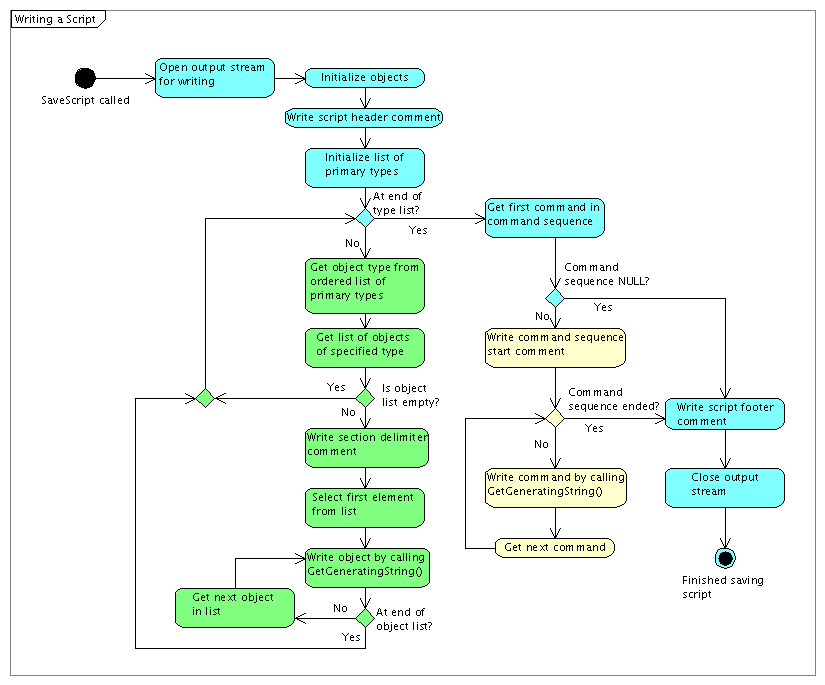
\includegraphics[430,357]{Images/WritingaScript.png}
% WritingaScript.png: 825x685 pixel, 72dpi, 29.10x23.81 cm, bb=0 0 825 685
\caption{\label{figure:WritingScriptFlow}Sequence Followed when Writing a Script}
\end{center}
\end{figure}

The procedure followed when writing a script file from GMAT is markedly simpler than that followed
when parsing a script file.  Figure~\ref{figure:WritingScriptFlow} shows the basic control flow
exercised when the ScriptInterpreter writes a script file.  First the ScriptInterpreter
initializes itself if it has not been initialized previously, and opens the output stream that is
the target of the script.  Then the ScriptInterpreter retrieves the configured items by type, and
writes these items to the output stream.  Comment lines are inserted at appropriate places during
this process, as indicated in the figure.  After all of the configured objects have been written,
the ScriptInterpreter walks through the command sequence, writing the commands out in order.  This
completes the script writing process.

\begin{figure}[htb]
\begin{center}
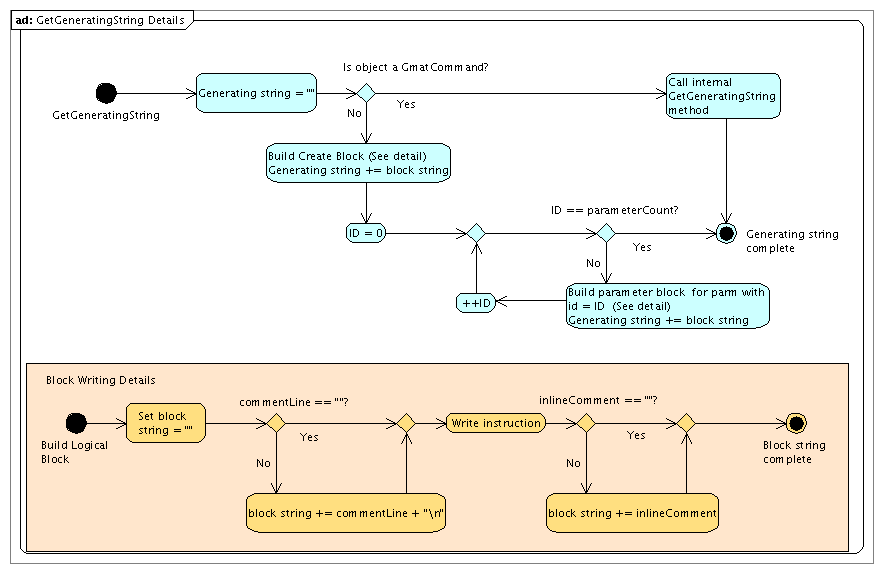
\includegraphics[400,260]{Images/GetGeneratingStringDetails.png}
\caption{\label{figure:ObjectGetGeneratingString}Sequence Followed by
\texttt{GmatBase::GetGeneratingString()} when Writing a Script}
\end{center}
\end{figure}

Script writing is significantly simplified because each user configurable object in GMAT includes a
method, \texttt{GetGeneratingString()}, which returns the full script string required to reproduce
the object.  This interface is included in the GmatBase class diagram,
Figure~\ref{figure:GmatBaseCommentInterface}.  The \texttt{GetGeneratingString()} method
essentially serializes any GMAT object derived from GmatBase (see
Section~\ref{section:GmatBase}).  When the \texttt{GetGeneratingString} function is called, the
object builds this string based on its internal data.  Command strings consist of a single
instruction, optionally decorated with preceding comments or inline comments.  Configured objects
build multi-instruction strings, consisting of an opening ``Create'' line and the assignment lines
required to set the internal object parameters.  Details of this process are shown in
Figure~\ref{figure:ObjectGetGeneratingString}.  The ScriptInterpreter just calls this method
sequentially on the objects to write the requested script.

This same facility is used at several other places in GMAT.  The MATLAB interface supports
serialization and passing of GMAT objects into MATLAB classes.  This support is also provided by the
\texttt{GetGeneratingString()} method.  Similarly, the GMAT graphical user interface includes a
popup window that shows scripting for all GMAT objects and commands.  The
\texttt{GetGeneratingString()} method is called to populate this window.

\section{\label{section:ScriptClasses}Classes Used in Scripting}

The preceding sections described the process followed when reading and writing scripts.  This
section outlines how those processes are implemented in GMAT.

\subsection{\label{section:ScriptInterpreter}The Script Interpreter}

The ScriptInterpreter is the class that manages the reading and writing of script files for GMAT.
It makes use of several helper classes when actually reading and writing scripts, along with core
Interpreter functions from the Interpreter base class.  Actions taken by the ScriptInterpreter can
be broken into two categories: script reading and script writing.  The complexity of these processes
is shown in Figures~\ref{figure:ReadingScriptFlow} and~\ref{figure:WritingScriptFlow}.  In this
section, the Interpreter and ScriptInterpreter classes are described, along with their helper
classes, the ScriptReadWriter and the TextParser.  These classes are shown in
Figure~\ref{figure:ScriptInterpreterClasses}.  Then the process followed to accomplish each of the
reading and writing tasks is presented. Script reading is particularly complex, so the script
reading procedure is broken into descriptions of the process followed for each of the four types of
script blocks GMAT supports.  The description of the class interactions performed when reading a
script can be found in Section~\ref{section:SIReadSequence}. The class interactions followed when
writing a script are outlined in Section~\ref{section:SIReadSequence}.

\begin{figure}[htb]
\begin{center}
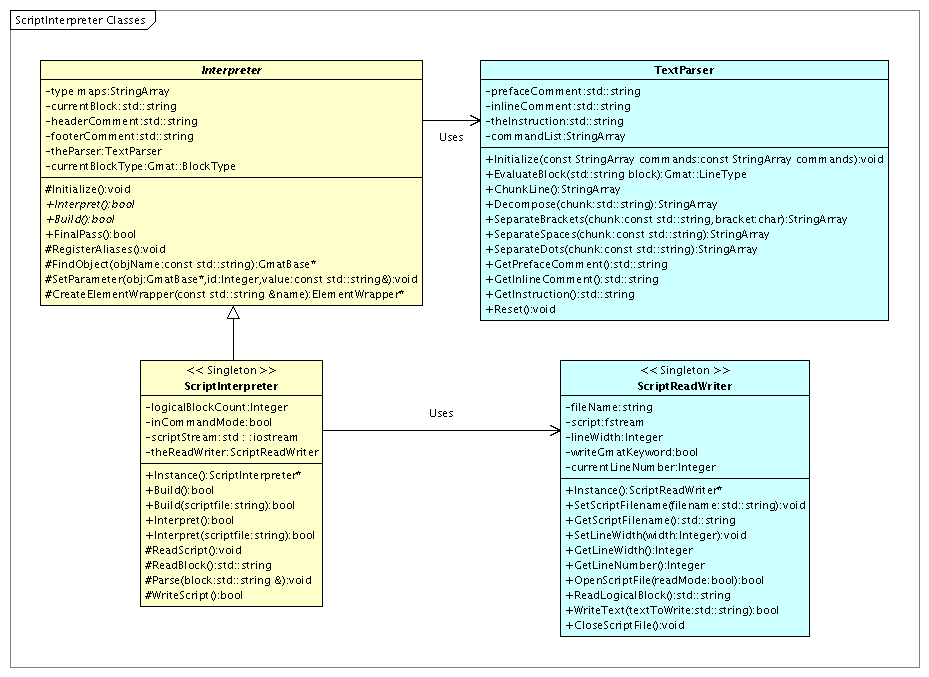
\includegraphics[400,292]{Images/ScriptInterpreterClasses.png}
\caption{\label{figure:ScriptInterpreterClasses}Classes in the ScriptInterpreter Subsystem}
\end{center}
\end{figure}

\subsubsection{Global Considerations}

The Interpreter subsystem used several components that exist at the program scope in GMAT.  There
are three enumerations used by the Interpreters that are defined in the Gmat namespace:

\begin{itemize}
\item \textbf{Gmat::ParameterType}: An enumeration used to identify the data type for internal
parameters in GmatBase derived objects.
\item \textbf{Gmat::WriteMode}: An enumeration that identifies the type of output requested from a
call to an object's GetGeneratingString() method.
\item \textbf{Gmat::BlockType}: An enumeration identifying the type of logical block parsed from a
script.
\end{itemize}

The first two of these enumerations, ParameterType amd WriteMode, are used in a fairly rigid manner
in the Interpreter subsystem.  ParameterTypes are used to determine how to access the internal data
on objects for reading and writing; the object is queried for the type of the internal parameter,
and that parameter is accessed accordingly.  For example, when a parameter value on an object
needs to be set, the Interpreter use the results of this query to call the correct set method on
the object -- SetRealParameter for floating point data, SetIntegerParameter for integers,
SetStringParameter for strings, and other calls for their corresponding types.

When calling the GetGeneratingString methods on objects, the Interpreters need to identify the style
of text that is required.  This style is identified using the identifiers in the WriteMode
enumeration.  The ScriptInterpreter uses the Gmat::SCRIPTING entry from this list.  Objects that
are passed to MATLAB use the Gmat::MATLAB\_STRUCT entry, and so forth.

The BlockType enumeration has four members: COMMENT\_BLOCK, DEFINITION\_BLOCK, COMMAND\_BLOCK, and
ASSIGNMENT\_BLOCK.  These members are used to identify the type of logical block parsed from a
script, as described in Section~\ref{section:SIReadSequence}.

\subsubsection{The ScriptInterpreter Class}

The ScriptInterpreter class manages the script reading and writing process.  Derived from the
Interpreter class, this singleton\footnote{See Section~\ref{section:TheSingletonPattern}} has
methods that use a ScriptReadWriter to open and close file streams and to use those streams to
perform the actions required to load and save GMAT scripts.  The entry point methods that take input
from the stream include the word ``Interpret'' in their names; the methods that launch the
serialization of GMAT objects and that subsequently write them out to streams use the work ``Build''
as part of the method name.

The key ScriptInterpreter data members and methods are described below.

\subparagraph{\textit{Class Attributes}}

\begin{itemize}
\item \textbf{Integer logicalBlockCount}: A counter that counts the logical blocks of script as
they are read.
\item \textbf{bool inCommandMode}: A flag that is used to detect when a script switches from object
parameter mode into command mode, so that assignment blocks can be configured correctly.
\item\textbf{std::iostream scriptStream}: The stream used for script reading or writing.
\item\textbf{ScriptReadWriter* theReadWriter}: A pointer to the ScriptReadWriter used when reading
or writing the script.
\end{itemize}

\subparagraph{\textit{Methods}}

\begin{itemize}
\item \textbf{ScriptInterpreter* Instance()}: The method used to obtain the pointer to the
singleton.
\item \textbf{bool Build()}: Method used to write a script to the stream.  This method calls
WriteScript() to perform the actual work required when writing a script.
\item \textbf{bool Build(const std::string \&scriptfile)}:  Method used to initialize the stream to
an output file.  This method calls Build() (above) after setting up the stream.
\item \textbf{bool Interpret()}: Method used to read a script from the stream.  This method calls
the protected ReadScript() method to perform the actual script reading tasks.
\item \textbf{bool Interpret(const std::string \&scriptfile)}:  Method used to initialize the stream
to an input file.  This method calls Interpret() (above) after setting up the stream.
\item \textbf{void ReadScript()}: The method that controls script reading.  This method is called by
Interpret().  The process followed in the ScriptInterpreter::ReadScript() method and the methods it
calls is shown in Figure~\ref{figure:InterpreterReadInteractionsTopLevel} and the diagrams derived
from it, and described in Section~\ref{section:SIReadSequence}.
\item \textbf{std::string ReadLogicalBlock()}: Method that obtains a logical block from teh
ScriptReadWriter for the ReadScript() method.
\item \textbf{void Parse(std::string \&block)}: Method that interprets a logical block for the
ReadScript() method.
\item \textbf{bool WriteScript()}: Control method used to write a script.  This protected method is
called by the Build() method when a script needs to be written.  The process followed in
the WriteScript() method is shown in Figure~\ref{figure:InterpreterWriteSequence} and
described in Section~\ref{section:SIWriteSequence}.
\end{itemize}

\subsubsection{\label{section:InterpreterBaseClass}The Interpreter Base Class}

The Interpreter base class defines the interfaces into the Interpreter system, and provides
functionality shared by all GMAT Interpreters. This class contains the data structures necessary to
manage data that exists at the mission scope rather than at object scope, like header and footer
comments.

\subparagraph{\textit{Class Attributes}}

\begin{itemize}
\item \textbf{StringArray type maps}: Lists of the names of classes of corresponding types of
configurable objects.  There are separate maps for commands (\textbf{commandMap}), hardware
components (\textbf{hardwareMap}), forces (\textbf{physicalmodelMap}), solvers (\textbf{solverMap}),
parameters (\textbf{parameterMap}), stopping conditions (\textbf{stopcondMap}), and
functions (\textbf{functionMap}).  These arrays are populated when the Interpreter is initialized.
\item \textbf{std::string currentBlock}: the current logical block of script, used while parsing.
\item \textbf{std::string headerComment}: The optional commentary, provided by the user, that
precedes all instructions in a GMAT mission.
\item \textbf{std::string footerComment}: The optional commentary, provided by the user, that
completes all instructions in a GMAT mission.
\item\textbf{TextParser theParser}: A TextParser used to pieces of text.
\item \textbf{enum currentBlockType}: An identifier for the type of the current logical block of
text, used when reading a script.
\end{itemize}

\subparagraph{\textit{Methods}}

\begin{itemize}
\item \textbf{void Initialize()}: Fills or refreshes the type maps by retrieving the lists of type
names from the Moderator.
\item \textbf{bool Interpret()}: Retrieves input from a stream and translates it into GMAT actions.
 This abstract method is implemented by all derived Interpreters.
\item \textbf{bool Build()}: Accesses GMAT objects and writes them to a stream. This abstract method
is implemented by all derived Interpreters.
\item \textbf{void FinalPass()}: Invoked after objects have been interpreted from a stream, this
method sets pointers for object references that are required outside of the Sandbox, so that
required functionality can be provided prior to initialization for a mission run.  Derived
Interperters should call this method as the last call in their Interpret() methods if internal
pointers are not set during execution of the method.
\item \textbf{void RegisterAliases()}: Some GMAT script identifiers can be accessed using multiple
text strings.  The RegisterAliases() method creates a mapping for these strings so that scripts are
parsed correctly.  The current GMAT system has five aliased parameter strings: ``PrimaryBodies''
and ``Gravity'' are both aliases for ``GravityField'' forces, ``PointMasses'' is an alias for `a
PointMassForce, ``Drag'' is an alias for a DragForce, and ``SRP'' is an alias for
SolarRadiationPressure.
\item \textbf{GmatBase* FindObject(const std::string objName)}: Method used to find a configured
object.
\item \textbf{void SetParameter(GmatBase *obj, const Integer id, const std::string \&value)}:
Method used to set parameters on configured objects.  Note that while the input value is a string,
it is converted to the correct type before being set on the object.
\item \textbf{\label{method:CreateElementWrapper}ElementWrapper* CreateElementWrapper(const
std::string \&name)}: Method used to create wrapper instances needed to use object properties,
Parameters, array elements, and other types of object data inside of the commands that implement the
Mission Control Sequence. The wrapper infrastructure is described in
Section~\ref{section:DataWrappers}.
\end{itemize}

\subsection{\label{section:ScriptReadWriter}The ScriptReadWriter}

File management tasks necessary to scripting are provided by the ScriptReadWriter class.  This
class, a singleton, is used by the ScriptInterpreter to retrieve script data a logical block at a
time and to write script files out on user request.  It does not directly interact with GMAT
objects; rather, it provides the interfaces into the file system that are used to store and retrieve
GMAT configurations in the file system.

\subparagraph{\textit{Class Attributes}}

\begin{itemize}
\item \textbf{std::string fileName}:  The current script name.
\item \textbf{std::fstream script}:  an std::fstream object used to read or write the script.
\item \textbf{Integer lineWidth}:  The maximum line width to use when writing a script; the
default width is 0 characters, which is treated as an unlimited line width.
\item \textbf{bool writeGmatKeyword}: A flag used to determine if the keywork GMAT is written when
a script file is written.  This flag defaults to true, and all assignment lines are prefaed with
the GMAT keyword.  Future builds of GMAT may toggle this feature off.
\item \textbf{Integer currentLineNumber}:  The current physical line number in the script file.
\end{itemize}

\subparagraph{\textit{Methods}}

\begin{itemize}
\item \textbf{TextReadWriter* Instance()}: Accessor used to obtain the pointer to the
TextReadWriter singleton.
\item \textbf{void SetScriptFilename(const std::string \&filename)}: Sets the name of the script
file.
\item \textbf{std::string GetScriptFilename()}: Gets the current name of the script file.
\item \textbf{void SetLineWidth(Integer width)}: Sets the desired line width.  If the input
parameter is less than 20 but not 0, GMAT throws an exception stating that line widths must either
be unlimited (denoted by a value of 0) or greater than 19 characters.
\item \textbf{Integer GetLineWidth()}: Gets the desired line width.
\item \textbf{Integer GetLineNumber()}: Gets the line number for the last line read.
\item \textbf{bool OpenScriptFile(bool readMode)}:  Opens the file for reading or writing, based on
the read mode (true to read, false to write).  This method sets the fileStream object to the
correct file, and opens the stream.
\item \textbf{std::string ReadLogicalBlock()}: Reads a logical block from the file, as described
below.
\item \textbf{bool WriteText(const std::string \&textToWrite)}: Writes a block of text to the
stream.  The text is formatted prior to this call.
\item \textbf{bool CloseScriptFile()}:  Closes the file if it is open.
\end{itemize}

\subsubsection{Overview of the ReadLogicalBlock() Method}

The ReadLogicalBlock() method is designed to handle ASCII files written from any supported platform
-- Windows, Macintosh, or Linux -- without needing to update the line ending characters.  This
method works by scanning each line for CR and LF characters, and treating any such character or
combination of characters found as a physical line ending character.  This process lets GMAT handle
text files on all of the supported platforms\footnote{Here's what the Computer Dictionary
(http://computing-dictionary.thefreedictionary.com/CR/LF) says about the line ending issue:
\begin{quote}
(Carriage Return/Line Feed) The end of line characters used in standard PC text files (ASCII
decimal 13 10, hex 0D 0A). In the Mac, only the CR is used; in Unix, only the LF. When one considers
that the computer world could not standardize the code to use to end a simple text line, it is truly
a miracle that sufficient standards were agreed upon to support the Internet, which flourishes only
because it is a standard.
\end{quote}
\noindent Linux follows the Unix convention.  Macintosh can be switched to Unix format or native
Macintosh format.}.

For the purposes of the ReadLogicalBlock() method, a logical block is one or more physical lines of
text in the script file, joined together into a single block of text.  A script file indicates that
physical lines should be connected by appending ellipsis (``...'') to indicate that a line is
continued.  For example, if this scripting is found in the file:
\begin{quote}
\begin{verbatim}
   Propagate Synchronized prop1(MMS), ...
      prop2(TDRS);
\end{verbatim}
\end{quote}
\noindent the encoded instruction that is returned is
\begin{quote}
\begin{verbatim}
   Propagate Synchronized prop1(MMS),        prop2(TDRS);
\end{verbatim}
\end{quote}

\noindent Note that the white space is preserved in this process.  The ellipsis characters are
replaced by a single space.

\subsubsection{ReadLogicalBlock(): Reading Comment Lines}

Comments related to specific GMAT objects need to be preserved when reading and writing script
files.  The comments associated with specific objects are considered as part of the object's logical
block.  Thus, expanding on the example above, if the scripting reads

\begin{quote}
\begin{verbatim}
   % Single step both formations
   Propagate Synchronized prop1(MMS), ...
      prop2(TDRS);
\end{verbatim}
\end{quote}
\noindent the logical block that is returned is two physical lines:
\begin{quote}
\begin{verbatim}
   % Single step both formations
   Propagate Synchronized prop1(MMS),        prop2(TDRS);
\end{verbatim}
\end{quote}

\noindent where the line break delimits the separation between the comment prefacing the command
from the text configuring the command object.  Similarly, inline comments are preserved as part of
the logical block; for example, the following scripting

\begin{quote}
\begin{verbatim}
   % Build the spacecraft
   Create Spacecraft Indostar1   % An Indonesian GEO
   % Set up a Geostationary orbit
   GMAT Indostar1.SMA = 42165.0    % Geosynchronous
   GMAT Indostar1.ECC = 0.0005     % Circular
   GMAT Indostar1.INC = 0.05       % Nearly equatorial
\end{verbatim}
\end{quote}
\noindent produces 4 logical blocks:

\begin{enumerate}
\item The object creation block:
\begin{quote}
\begin{verbatim}
   % Build the spacecraft
   Create Spacecraft Indostar1   % An Indonesian GEO
\end{verbatim}
\end{quote}
\item The first parameter setting block, with 2 comments:
\begin{quote}
\begin{verbatim}
   % Set up a Geostationary orbit
   GMAT Indostar1.SMA = 42165.0    % Geosynchronous
\end{verbatim}
\end{quote}
\item a second parameter block:
\begin{quote}
\begin{verbatim}
   GMAT Indostar1.ECC = 0.0005     % Circular
\end{verbatim}
\end{quote}
\item and the final parameter block:
\begin{quote}
\begin{verbatim}
   GMAT Indostar1.INC = 0.05       % Nearly equatorial
\end{verbatim}
\end{quote}
\end{enumerate}

There are three additional types of comment blocks that the ReadLogicalBlock() method manages.
These blocks, (1) the script header, (2) the script footer, and (3) section delimiter blocks, are
not associated with specific GMAT objects, but rather with the script file as a whole.

GMAT script header comments are comment lines that begin on the first line of the script file, and
that are terminated by a blank line.  An example, taken, with minor edits, from one of the GMAT test
scripts, is shown here:

\begin{quote}
\begin{verbatim}
% GMAT Script File
% GMAT Release Build 6.0, February 2006
%
% This test script uses the GMAT script language to convert from
% the Cartesian to the Keplerian state.  I only implemented the
% conversion for elliptic inclined orbits, as described in the
% math spec.  I didn't implement other special cases, because it
% would not test anything different in the inline math.


%  Create a s/c
Create Spacecraft Sat;
...
\end{verbatim}
\end{quote}

\noindent This script snippet contains a header comment, read into the logical block

\begin{quote}
\begin{verbatim}
% GMAT Script File
% GMAT Release Build 6.0, February 2006
%
% This test script uses the GMAT script language to convert from
% the Cartesian to the Keplerian state.  I only implemented the
% conversion for elliptic inclined orbits, as described in the
% math spec.  I didn't implement other special cases, because it
% would not test anything different in the inline math.
\end{verbatim}
\end{quote}

\noindent and an object creation logical block:

\begin{quote}
\begin{verbatim}
%  Create a s/c
Create Spacecraft Sat;
\end{verbatim}
\end{quote}

The script header comment is stored in the headerComment data member of the ScriptInterpreter.  The
comment associated with the object creation logical block is stored with the associated object, as
described in the next section.

Some script files include comments after the last executable line of the script file.  When such
comments are found, they are collected into a single logical block and stored in the
ScriptInterpreter's footerComment data member.  The stored data in the header and footer comment
blocks are written in the appropriate locations when a script file is saved using the Build() method
of the ScriptInterpreter.

The final category of script comments, the section delimiters, are automatically generated when
writing a script file, and ignored when reading a script.  An example of a section delimiter is
shown here:

\begin{quote}
\begin{verbatim}
Create ImpulsiveBurn LunarPhasedV;
GMAT LunarPhasedV.Origin = Earth;
GMAT LunarPhasedV.Axes = VNB;
GMAT LunarPhasedV.VectorFormat = Cartesian;
GMAT LunarPhasedV.V = 0.027;

%--------------------------------------------------------------------------
%------------------------------ Propagators -------------------------------
%--------------------------------------------------------------------------

Create ForceModel LunarSB_ForceModel;
GMAT LunarSB_ForceModel.CentralBody = Earth;
GMAT LunarSB_ForceModel.PointMasses = { Earth, Sun, Luna};
\end{verbatim}
\end{quote}

\noindent Section delimiter comments exist on single lines, and always start with the string
\begin{quote}
\begin{verbatim}
%--------
\end{verbatim}
\end{quote}

\noindent with no preceding white space.   When the ReadLogicalBlock() method encounters this string
of characters at the start of a physical line, the physical line is ignored.

The ScriptInterpreter takes these logical blocks from the ScriptReadWriter, and uses the TextParser
class to process each logical block.  The facilities implemented in the TextParser and used for this
processing are described next.

\subsection{\label{section:TextParser}The TextParser Class}

The ScriptReadWriter provides the interface to script files, and includes a method,
ReadLogicalBlock(), that accesses a script file and reads it one logical block at a time.  The
ScriptInterpreter uses this method to obtain each logical block of text from a script.  When
ReadLogicalBlock() returns a script block, the ScriptInterpreter begins a process of breaking the
block into pieces until the entire block has been consumed and interpreted into internal GMAT data
structures.  The ScriptInterpreter uses the TextParser to perform this decomposition.

The TextParser class is used to process logical blocks of script, breaking them into their
constituent parts so that the Interpreters and Commands can setup the underlying class relationships
and parameter values needed to model the mission described in the script file.

The TextParser class provides methods used by the ScriptIntererpter to iteratively decompose a
logical block of text.  This class supplies all of the low level parsing functionality necessary to
manage script lines, and is used both by the ScriptInterpreter and by other classes -- notably
commands that are too complex to be treated generically.  The TextParser does not parse inline
mathematics; when inline math is detected by the ScriptInterpreter, it hands the parsing task off
to the MathParser, described in Chapter~\ref{chapter:InlineMath}.

\subparagraph{\textit{Class Attributes}}

\begin{itemize}
\item \textbf{std::string prefaceComment}: All comment lines that precede the instruction in the
current block of text.  This member is the empty string if there are no comment lines preceding the
instruction.
\item \textbf{std::string inlineComment}: Any comment text that is appended to the instruction.
This member is the empty string if there is no comment lines following the instruction.
\item \textbf{std::string theInstruction}: The text that is decomposed to tell GMAT what to do.
\item \textbf{StringArray commandList}: The list of available commands, excluding the GMAT keyword,
which is used for assignments.
\end{itemize}

\subparagraph{\textit{Methods}}

\begin{itemize}
\item \textbf{void Initialize(const StringArray \&commandList)}: Method that sets up the internal
data for the TextParser.  The parser's owner calls this method during construction, identifying all
of the commands available to the parser in the current scope.
\item \textbf{Gmat::LineType EvaluateBlock(const std::string \&block)}: The method that takes a
logical block and breaks it into three pieces: preface comments, the instruction in the block, and
inline comments.  These pieces are stored in internal TextParser data members until needed by the
ScriptInterpreter.  The method returns the type of block found, using these rules:
\begin{enumerate}
\item If theInstruction is empty, the block is a COMMENT\_BLOCK, otherwise
\item If theInstruction has the word ``Create'' as the opening word, it is a DEFINITION\_BLOCK,
otherwise
\item If theInstruction has a member of the commandList as the opening word, it is a COMMAND\_BLOCK,
otherwise
\item The line is an ASSIGNMENT\_BLOCK\footnote{Note that identifying a line as an assignment line
means that it will be used either to set an internal object parameter or to build an Assignment
command in the mission sequence.}.
\end{enumerate}
\item \textbf{StringArray ChunkLine()}: Breaks the instruction string into logical groups, called
``chunks'' in this document.  The instruction line is broken at white space and comma characters.
Blocks marked with the grouping delimiters (), \{\}, and [] are kept together as independent chunks.
\item \textbf{StringArray Decompose(std::string chunk)}: Breaks a text chunk into its constituent
pieces, and returns them in a StringArray.  This method is used to take a chunk from the
ChunkLine() method, and break it into substrings.  Decompose calls into the Separate methods
described below, looking first for brackets to break apart, then commas and spaces, and finally
periods.
\item \textbf{StringArray SeparateBrackets(const std::string \&text, const char bracket)}: Finds the
text in a bracket grouping, and separates it into its constituent pieces.  These pieces are returned
in a StringArray.  The first element of the array is the opening bracket, and the last element is
the closing bracket.
\subitem \textbf{text}: The string that contains the bracketed text.
\subitem \textbf{bracket}: The opening bracket type; this is one of the following characters: '(',
'\{', '[', or '<'.
\item \textbf{StringArray SeparateSpaces(const std::string chunk)}: Separates the chunk into pieces
at whitespace and comma characters.
\item \textbf{StringArray SeparateDots(const std::string chunk)}: Separates the chunk into pieces
at period (aka ``dot'') characters.
\item \textbf{std::string GetPrefaceComment()}: Accessor method used to get the preface comment
from the logical block.  If no preface was available, the method returns the empty string.
\item \textbf{std::string GetInlineComment()}: Accessor method used to get the inline comment
from the logical block.  If no inline comment was available, the method returns the empty string.
\item \textbf{std::string GetInstruction()}: Accessor method used to get the instruction
from the logical block.  If no instruction was available, the method returns the empty string.
\item\textbf{void Reset())}: Clears the internal data in the TextParser.
\end{itemize}

\section{\label{section:SIReadSequence}Call Sequencing for Script Reading and Writing}

The class descriptions described above provide a static picture of the components used to configure
GMAT to run a script and to save a script for later use.  In this section, the sequence followed
for script reading and writing is presented to show how the structures and methods described for
the classes interact with GMAT.

\subsection{Script Reading Call Sequence}

Script reading is the process through which the instructions in a script are translated into
internal object configuration in GMAT.  This process is, of necessity, rather complicated.
However, the division of the types of lines that a script can contain into four sets: comment
blocks, object definition blocks, command blocks, and assignment blocks, makes it possible to break
the process into more manageable pieces.  Accordingly, this section provides a top level look at
the process followed when reading a script, followed by a description of the sequence executed for
each type of logical block.

\subsubsection{Process Followed for All Logical Blocks.}

\begin{figure}
\begin{center}
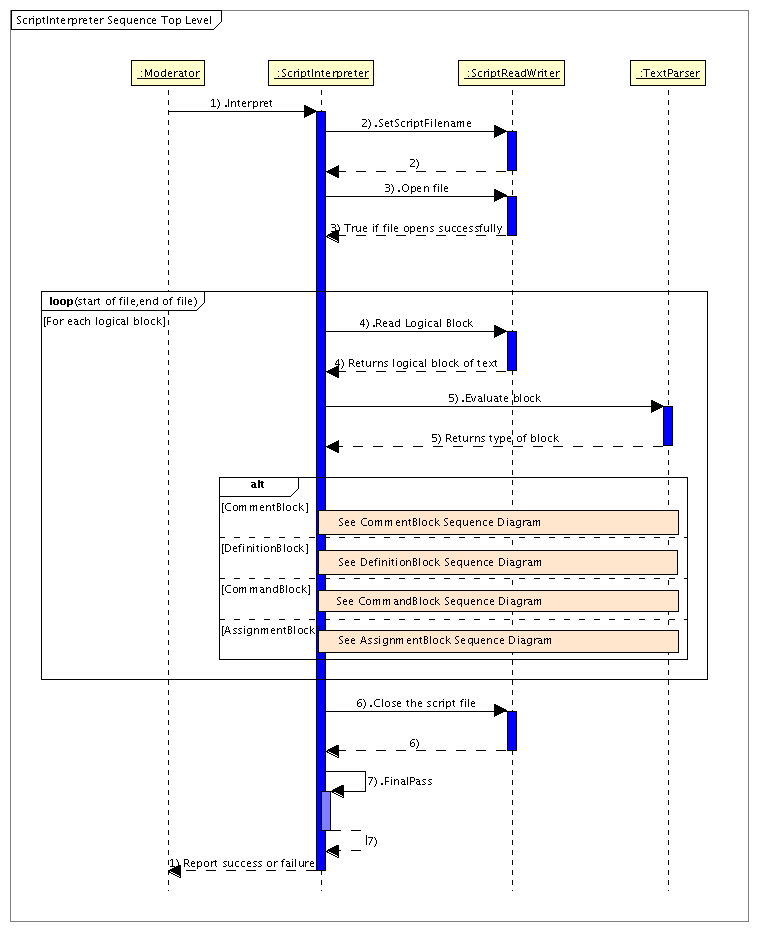
\includegraphics[400,491]{Images/ScriptInterpreterSequenceTopLevel.png}
\caption{\label{figure:InterpreterReadInteractionsTopLevel}Overview of Interpreter Class
Interactions when Reading a Script}
\end{center}
\end{figure}

When the ScriptInterpreter is instructed to read a script, it performs some basic
initialization in preparation for a new script file.  The headerComment and footerComment bata
members are set to empty strings, the logicalBlockCount data member is set to zero, the the
TextParser owned by the ScriptInterpreter is reset to prevent inadvertent use of data from a
previous script.  Once these preliminary actions are completed, the script can be read.

Figure~\ref{figure:InterpreterReadInteractionsTopLevel} shows the sequence followed when the
ScriptInterpreter reads a script.  The ScriptInterpreter sends the ScriptReadWriter the name
of the script that needs to be read, and then requests that the script be opened for reading.
If these commands succeed, the ScriptInterpreter uses the ScriptReadWriter to read the file, one
logical block at a time.

The ScriptInterpreter calls the TextParser::EvaluateBlock method with each block of script that it
receives from the ScriptReadWriter.  That method breaks the logical block into three pieces: the
comment lines that precede the instruction in the block, the instruction that needs to be
interpreted to configure GMAT, and any inline comments that appear in the block.  The TextParser
examines the instruction portion of the block to determine what type of instruction is encoded in
the block, and returns the type information using the LineType enumeration from the Gmat namespace.

The ScriptInterpeter then initiates actions that translate the block into components used to
setup the script instructions, based on the type of block that was detected.  The process foloowed
for the four possible types of script line are detailed in the sections that follow this one, and
illustrated in Figures~\ref{figure:InterpreterReadInteractionsCommentBlock} --
\ref{figure:InterpreterReadInteractionsAssignmentBlock}.

Once the ScriptInterpreter has processed all of the blocks from a script, it instructs the
ScriptReadWriter to close the script.  The ScriptInterpreter then executes a final pass through the
objects in the current configuration, setting a minimal set of object cross references that are
required to make GMAT's GUI functional.  When this final pass has been performed, control is
returned to the Moderator with all of the instructions encoded in the script translated into GMAT
objects.

The following paragraphs describe the details executed when translating each of the types of
logical blocks that GMAT scripts use.

\subsubsection{Comment Blocks}

\begin{figure}[htb]
\begin{center}
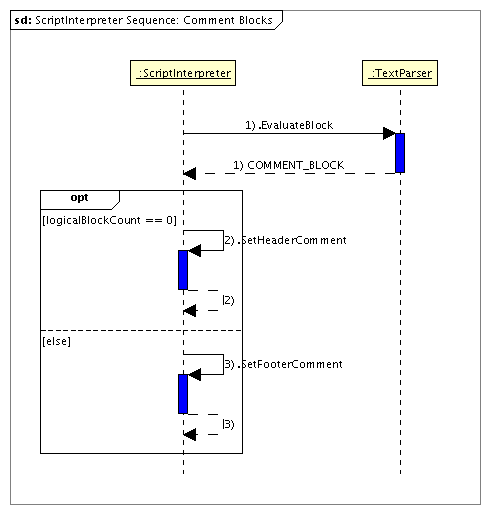
\includegraphics[280,294]{Images/ScriptInterpreterSequenceCommentBlocks.png}
\caption{\label{figure:InterpreterReadInteractionsCommentBlock}Interpreter Class Interactions when
Reading a Comment Block}
\end{center}
\end{figure}

The only time the ScriptReadWriter returns a comment block -- that is, a block of script that has
no instructions, and consists only of comments -- is when the block is either the header comment
for the script or the footer comment for the script.  Script files do not necessarily have either
of these blocks.  The ScriptInterpreter maintains an internal counter tht it uses to count the
logical blocks as they are read from the file.  If that counter is zero and a comment block is
found, then the block is the header comment; otherwise it is the footer comment.
Figure~\ref{figure:InterpreterReadInteractionsCommentBlock} shows this sequence.

\subsubsection{Object Definition Blocks}

\begin{figure}
\begin{center}
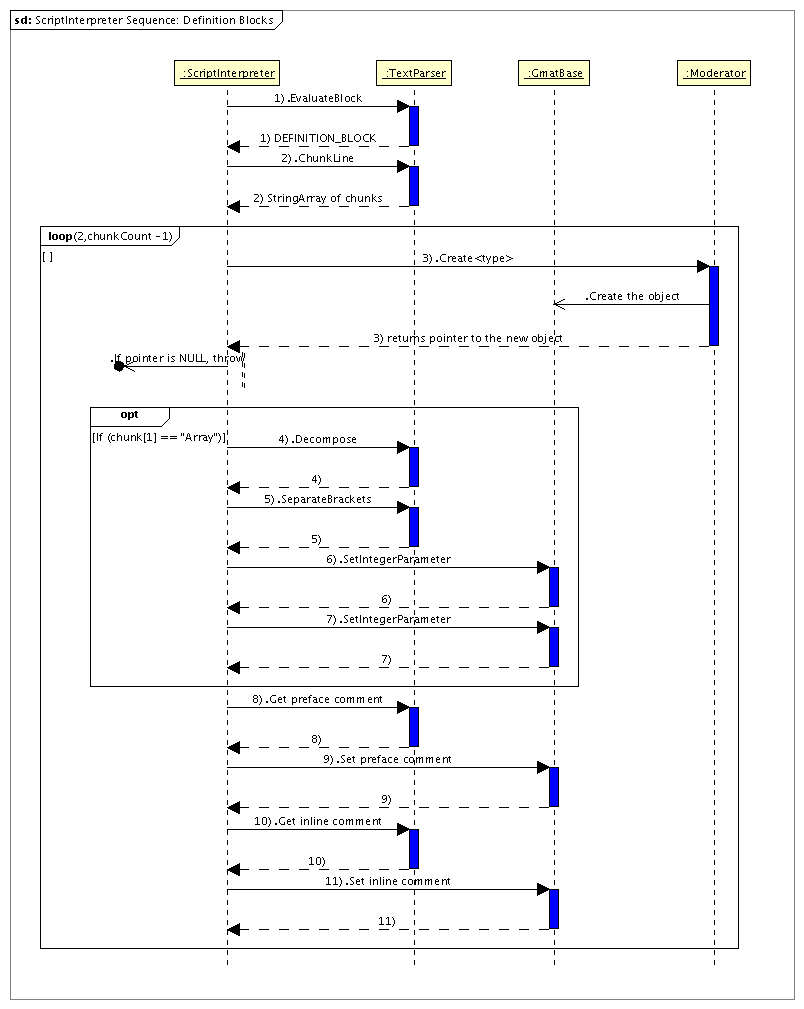
\includegraphics[400,502]{Images/ScriptInterpreterSequenceDefinitionBlocks.png}
\caption{\label{figure:InterpreterReadInteractionsDefinitionBlock}Interpreter Class Interactions
when Reading an Object Definition Block}
\end{center}
\end{figure}

``Create'' lines an a script file invoke object definition instructions, which are processed
following the sequence shown in Figure~\ref{figure:InterpreterReadInteractionsDefinitionBlock}.
These instructions instantiate the user configurable objects that are used to model a mission.

When the TextParser tells the ScriptInterpreter that an object definition block has been detected,
the ScriptInterpreter asks the TextParser to break the instruction in the block into smaller
pieces, referred to as chunks.  The text parser breaks the instruction at each white space or
comma character in the instruction, and places these pieces, in order, into a StringArray,
referred to here as the ``chunkArray.''  Once the instruction has been broken into chunks, the
chunkArray is returned to the ScriptInterpreter for processing.

Object definition instructions all have the format

\begin{quote}
   \texttt{Create <ObjectType> <Name1>[, <Name 2>, ...]}
\end{quote}

\noindent where ObjectType is a string identifying what type of object is desired -- examples are a
Spacecraft, a ForceModel, a Propagator, an Array, and so on.  The instruction has one or more
object names; one object will be created for each name found in the instruction.  Object names
start at the third element in the chunkArray, chunkArray[2].  If the size of the chunkArray is less
than 3, the ScriptInterpreter throws an exception stating that no object name was found in the
object definition line.

The object names in the instruction text are separated by commas, white space, or both.  The Array
object type has, in addition, a block specifying the array's dimensions, contained in square
brackets. The array dimensions are written to a separate chunk in the chunkArray, starting from the
opening square bracket (``['') and ending with the closing bracket (``]''), when the instruction is
broken into pieces.

Once the instruction has been broken into chunks, the ScriptInterpreter starts to loop through the
list of object names found in the chunkArray.  For each object name, it calls the Moderator to
create an instance of the object.  The Moderator returns a pointer to the new object, which the
ScriptInterpreter checks.  If the pointer is NULL, the ScriptInterpreter throws an exception
stating that a requested object could not be created.  This exception includes the name of the
object, the object type, and the text of the instruction that attempted to create the object.  If
the returned pointer was not NULL, the ScriptInterpreter continues processing.

If the object created was an Array, the ScriptInterpreter takes the next chunk from the chunkArray,
and asks the TextParser to break the bracketed dimensions apart.  These dimensions are then passed
into the new Array object to set the number of rows and columns for the array.

Finally, the ScriptInterpreter sets the comment strings for the new object by accessing the preface
and inline pieces in the TextParser, and passing those pieces into the object.  This completes the
configuration of the object, so the ScriptInterpreter requests the next name from the chunkArray.
It then repeats the process until all of the named objects have been created.

\subsubsection{\label{section:ParsingCommandBlocks}Command Blocks}

\begin{figure}
\begin{center}
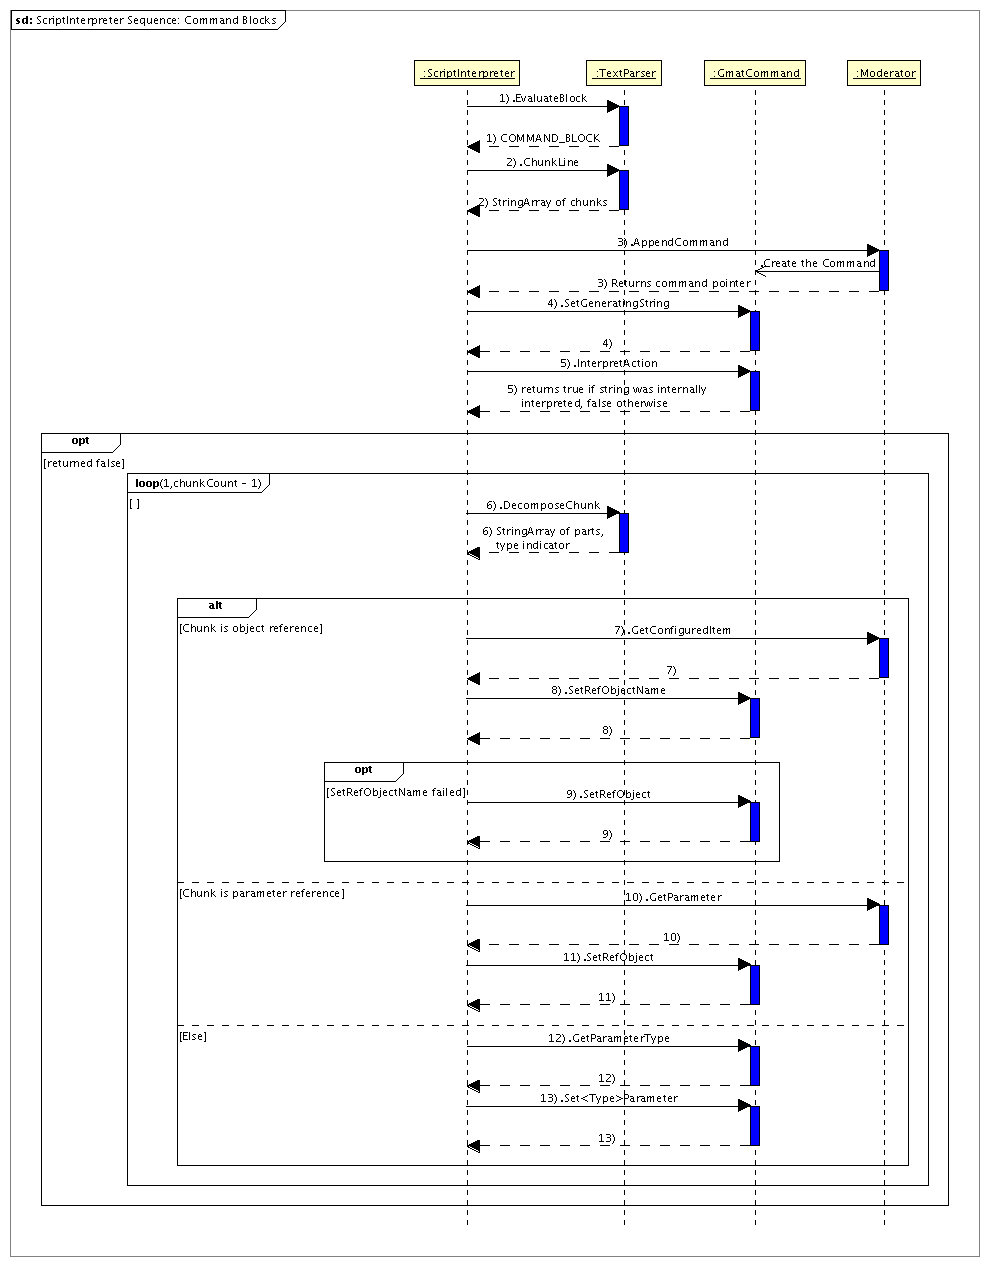
\includegraphics[400,512]{Images/ScriptInterpreterSequenceCommandBlocks.png}
\caption{\label{figure:InterpreterReadInteractionsCommandBlock}Interpreter Class Interactions when
Reading a Command Block}
\end{center}
\end{figure}

The time ordered sequence of events executed when GMAT runs a mission sequence are encoded in
commands -- objects that instantiate the classes derived from the GmatCommand class, as described
in Chapter~\ref{chapter:Commands}.  Figure~\ref{figure:InterpreterReadInteractionsCommandBlock}
shows the sequence of events that is followed by the Script Interpreter when a command is
configured.  The first command detected by the script interpreter toggles the ScriptInterpreter's
inCommandMode flag on, and sets the flag in the ScriptReadWriter so that all subsequent assignment
blocks are treated as Assignment commands.

When a command is detected and set for configuration, the ScriptInterpreter calls the Moderator
and asks for an instance of the command.  It then sets the generating string on the command.  Some
commands parse the generating string internally, using the bool InterpretAction() method.  Commands
that use this method create an instance of the TextParser, and use its public methods to decompose
the string into its constituent pieces.  An example of this type of command is the Propagate
command, which has a generating string that can consist of many different options.  The complexity
of the command makes it difficult to handle in a generic fashion in the ScriptInterpreter; hence it
provides the parsing service internally.  Commands that perform internal parsing return a value of
``true'' from the call to InterpretAction; those that expect to be configured by the
ScriptInterpreter return ``false.''

If the command is not parsed internally, the instruction line is broken into chunks, using the
cams call as performed for object definition.  The resulting chunks are the command components
needed to configure the command.  The instruction components embedded in a GMAT command line
typically exist in one of several different forms:

\begin{enumerate}
\item Stand alone commands.  Some commands take no parameters at all, and are simply added to the
command list unadorned.  An example of this type of command is the EndTarget command, which
identifies the end of a targeting loop.
\item Lists of referenced objects, separated by white space or commas.  An example of this type of
command is the Save command, which has the format
\begin{quote}
\begin{verbatim}
   Save <objectName>
\end{verbatim}
\end{quote}
\noindent When a Save command is encountered, the name of the object is passed to the command using
the SetReferenceObjectName()) method.
\item Lists of parameters, separated by white space or commas.  An example of this type of
command is the Report command, which has the format
\begin{quote}
\begin{verbatim}
   Report reportObject parameter1 parameter2 ...
\end{verbatim}
\end{quote}
\noindent When a Report command is encountered, the name of the items in the list are passed
to the command using the SetRefObject() method.  The command validate teh first object as a
ReportFile instance, and the subsequent objects as parameters.
\item Objects with references.  Some commands identify objects that have associated objects.  An
example of this type of command is the BeginFiniteBurn command, which has the format
\begin{quote}
\begin{verbatim}
   BeginFiniteBurn <burnName>(<spacecraftName>)
\end{verbatim}
\end{quote}
\noindent The objects identified on this line are accessed from the Moderator, and passed into the
command as reference objects.
\end{enumerate}

Once these components have been set on the command, the ScriptInterpreter sets the comment strings
for the new object by accessing the preface and inline pieces in the TextParser, and passing those
pieces into the object.  This completes the configuration of the command, so the ScriptInterpreter
requests the next name from the chunkArray.  It then repeats the process until all of the named
objects have been created.

\subsubsection{Assignment Blocks}

\begin{figure}
\begin{center}
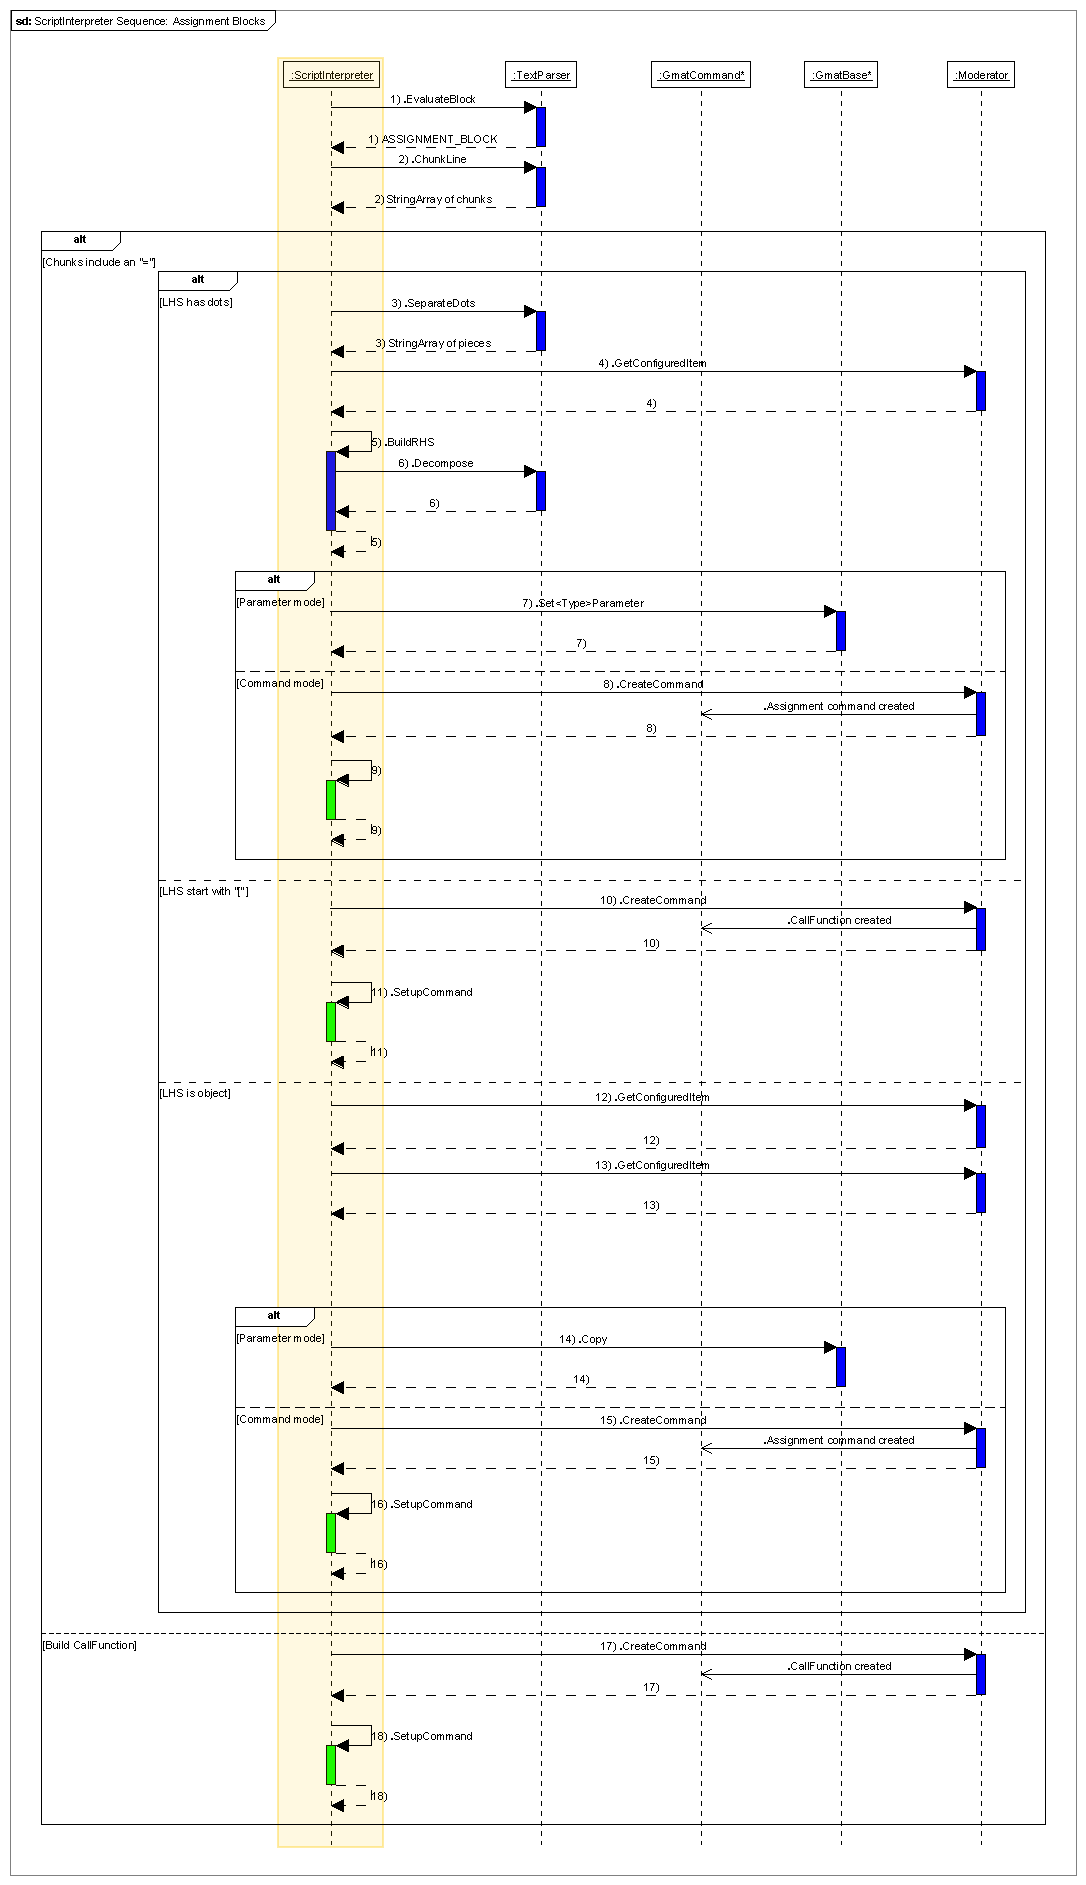
\includegraphics[331,575]{Images/ScriptInterpreterSequenceAssignmentBlocks.png}
\caption{\label{figure:InterpreterReadInteractionsAssignmentBlock}Interpreter Class Interactions
when Reading an Assignment Block}
\end{center}
\end{figure}

All logical blocks that are not comment blocks, object definitions, or commands are assignment
blocks\footnote{Assignment lines in the current scripting for GMAT all start with the text string
``GMAT''.  Since the ScriptInterpreter treats assignment lines last in the parsing sequence, this
string is now optional, though recommended for any scripts that will be read in MATLAB to avoid
confusing that system.}.  Processing for these blocks is shown in
Figure~\ref{figure:InterpreterReadInteractionsAssignmentBlock}.  The result of parsing an assignment
block can be either a changed value in a configured object or a new command inserted into the
mission sequence, depending on the setting of the inCommandMode flag.  If the assignment line
includes a function call or inline mathematics, the ScriptInterpreter automatically switches into
command mode and an appropriate command is created.

All assignment lines consist of an object identifier, and an optional equals sign followed by a
right side expression (typically referred to as the ``right hand side'', or RHS).  The only
assignment lines that are missing the equals sign are function calls, which execute a CallFunction
command. Assignment lines fall into the following categories:

\begin{enumerate}
\item Object properties.  Object property assignments are used to set the internal data on
configured objects.  Object properties can be set to constant values, the current values of
variables, or the value of an array element.
\item Objects.  Objects can be set equal to other objects of the same type.  When this form of
assignment is used, the Copy() method of the object on the left side of the assignment is called
with the object on the right as the input parameter.
\item Function calls.  Function call lines are used to execute GmatFunctions and MatlabFunctions.
\item Mathematics.  Scripted mathematics, as described in Chapter~\ref{chapter:InlineMath}, are also
managed on assignment lines.
\end{enumerate}

Figure~\ref{figure:InterpreterReadInteractionsAssignmentBlock} shows the sequence of function calls
required to interpret assignment lines.  The command configurations segments, shown in green on the
figure, execute the sequence described in the preceding section and shown on
Figure~\ref{figure:InterpreterReadInteractionsCommandBlock}.

\subsection{\label{section:SIWriteSequence}Script Writing Call Sequence}

\begin{figure}
\begin{center}
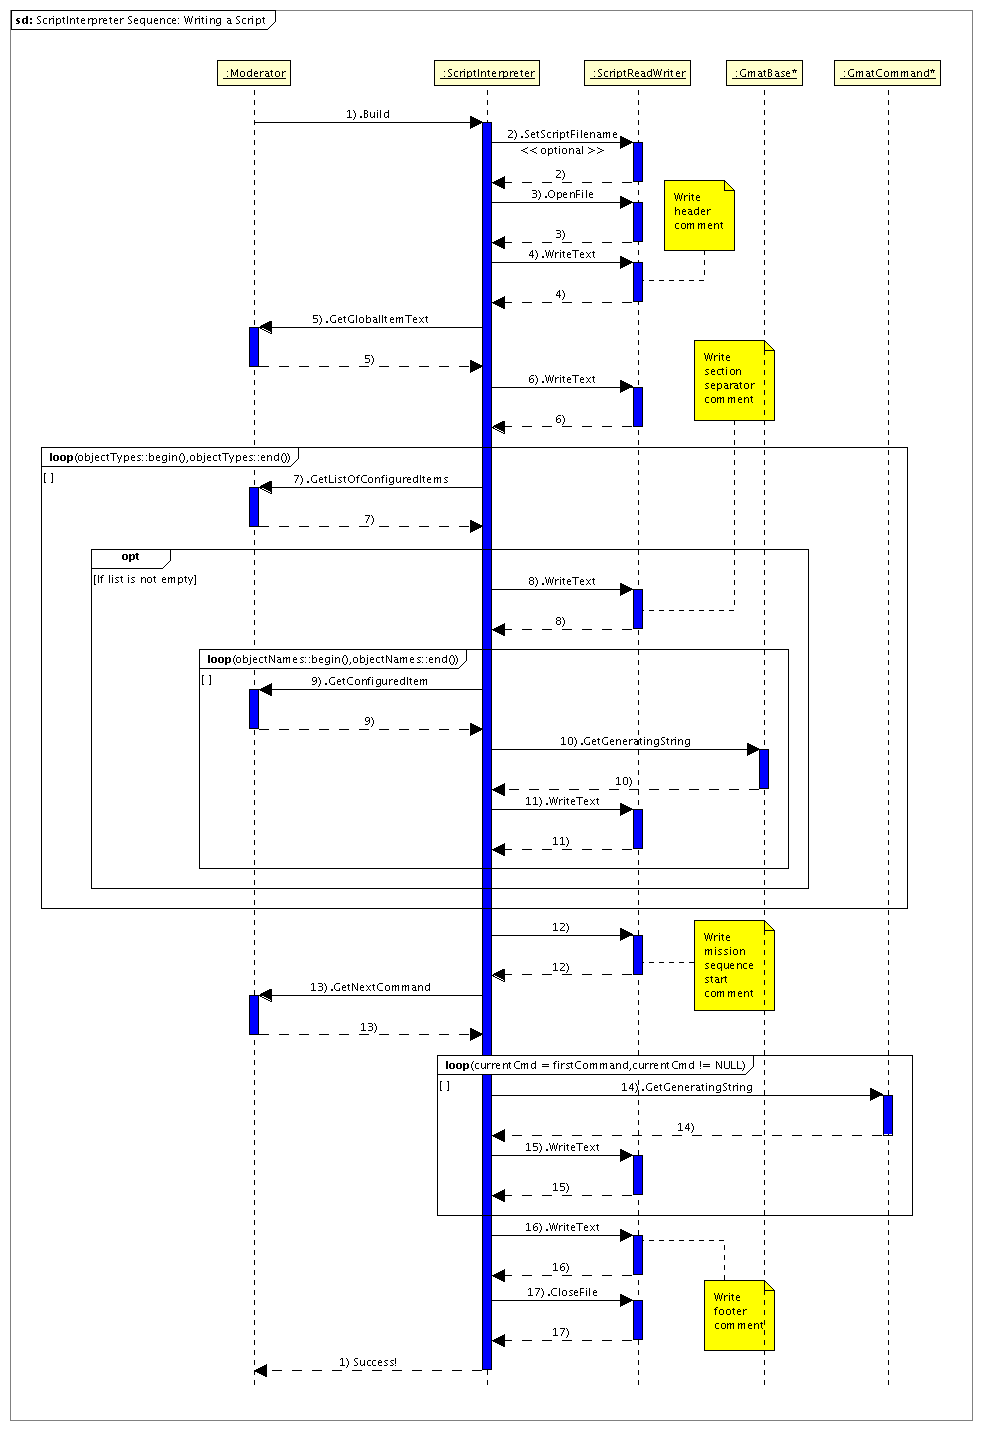
\includegraphics[395,575]{Images/ScriptInterpreterSequenceWritingaScript.png}
\caption{\label{figure:InterpreterWriteSequence}Calls Made when Writing a Script}
\end{center}
\end{figure}

The script writing process is considerably simpler than the reading process because all of the
objects that need to be written to script already exist and are configured to meet the user's
needs.  Figure~\ref{figure:InterpreterWriteSequence} shows the interactions performed between the
GMAT classes when a script is written.

A script writing sequence is initiated then the Moderator calls the Build(std::string nameOfFile)
method on the ScriptInterrpeter.  If the nameOfFile parameter in the Build() call is not the empty
string, then the ScriptInterpreter sets the script file name on the ScriptReadWriter to the name
passed in with the call.  Next the script is opened as an output stream.  The header comment is
written to the stream, followed by any global model information contained in the current GMAT
run\footnote{The global information currently consists of the flags used by the SolarSystem to
control the update intervals for planetary positions and the Earth nutation matrix.  The Moderator
call, GetGlobalItemText(), listed here returns the result of calling GetGeneratingString on the
current SolarSystem.  This method needs to be added to the Moderator.}.

After all of these preliminary data have been written, the ScriptInterpreter writes the configured
objects stored in the ConfigurationManager to the script stream.  These configured objects are
accessed by type, so that the resulting script presents the objects in sections based on the object
type.  The ScriptInterpreter calls the Moderator to get the list of objects by type.  If the list
is empty for a given type, the ScriptInterpreter skips to the next type.  Each block of objects is
prefaced by a section delimiter comment (as shown above). The section delimiters are generated
internally in the ScriptInterpreter when it determines that there is an object of a specified type
that needs to be written.

Configured objects are written in the following order: spacecraft, hardware, formations, force
models, propagators, Burns, variables and arrays, coordinate systems, solvers, subscribers (plots,
views and reports), and functions.  Each configured object supplies its own serialized description,
encoded in an std::string.  This string is accessed using the object's GetGeneratingString()
method; the ScriptInterpreter calls GetGeneratingString, and sends the resulting string to the
ScriptReadWriter, which writes it to the script stream.

Once all of the configured objects have been written to the output stream, the ScriptInterpreter
sends the block delimiter for the mission sequence to the ScriptReadWriter.  The ScriptInterpreter
then accesses the starting command in the mission sequence by calling the GetNextCommand() method
on the Moderator.  Since the command sequence is a linked list of GmatCommand objects, the
ScriptInterpreter no longer needs to access the Moderator for command information.  It sets an
internal pointer to the first command in the list.  This pointer, the current command pointer,
is used to call GetGeneratingString() on that command.  The returned string is passed to the
ScriptReadWriter, which writes it to the script stream.  The ScriptInterpreter then accesses the
next command in the sequence by calling the Next() method.  This process repeats as long as the
pointer returned from the call to Next() is not NULL.

BranchCommands automatically include the string data for their branches when their
GetGeneratingString() method is called.  The ScriptInterpreter does not have any special code that
needs to be run when a BranchCommand appears in the command sequence.

Once all of the commands in the command sequence have been written to the script stream, the
ScriptInterpreter sends the footer comment to the TextReadWriter, which writes out the footer com
ment.  The ScriptInterpreter then tell the ScriptReadWriter to close the script stream, completing
the script write function.


\section{\label{section:InterpretingGmatFunctions}Interpreting GMAT Functions}

GMAT scripting includes the ability to load and run smaller blocks of script using the GmatFunction
class described in Section~\ref{section:GmatFunctions}.  This functionality is managed and driven
by the CallFunction command and the GmatFunction class.  The Interpreter subsystem provides a
public base class method,
\begin{quote}
Interpreter::InterpretSubsequence(GmatFunction *function),
\end{quote}
\noindent that builds the control sequence for the GmatFunction.  This section describes how that
method works.  Figure~\ref{figure:InterpretGmatFunction} shows the basic flow followed in this
process.

\begin{figure}[htb]
\begin{center}
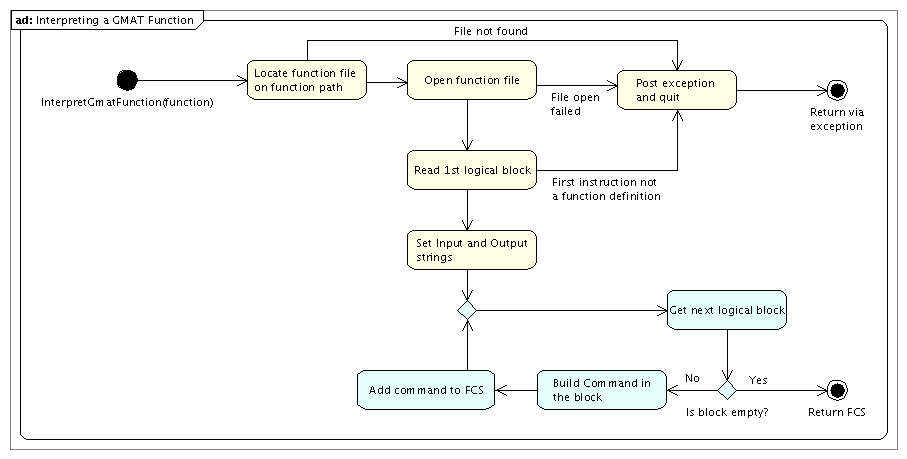
\includegraphics[454,230]{Images/InterpretingaGMATFunction.png}
\caption{\label{figure:InterpretGmatFunction}Interpreting a Function Control Sequence}
\end{center}
\end{figure}


<Text to be completed.>